\documentclass{article}

\usepackage{graphicx}

\title{World In A Word 2013 Competition:\\
Evolving Parameters for a Cayley Graph Visualiser Using 64 bits}
\author{Miguel Nicolau\\
NCRA group, UCD CASL\\
University College Dublin
\and Dan Costelloe\\
NCRA group, UCD CASL\\
University College Dublin}

\date{}

\begin{document}
\maketitle
\begin{abstract}
A 64-bit string evolved with a custom-built GA is mapped using the Grammatical
Evolution system, to evolve parameters for a visualiser of Cayley graphs.The
resulting visualisations, albeit restricted, still exhibit a large degree of
complexibility and evolvability, and are representative of the domain.
\end{abstract}

\section{Introduction}
The ``World in a Word'' 64-Bit Design Challenge is a competition run for the
IEEE Congress on Evolutionary Computation. The objective is to evolve 64-bit
strings, which are used to explore creative domains. Entries are evaluated
based on the originality of the domain, the diversity of the structures
evolved, the appeal of the domain and the evolved individuals, and the extent
to which the 64 bits are used.

This entry uses the 64 bits as a basis to create an integer string, which in
turn is used with the Grammatical Evolution system \cite{oneill03b}, to
evolve parameters for Jenn3d \cite{obermeyer10a}, a visualiser of Cayley graphs of
finite Coxeter groups. The mapping process is regulated through a context-free
grammar, which defines the parameter space to navigate.

The resulting system creates fully-formed images from the start, and adapts
quickly to the changing styling preferences of the user. The use of 64 bits
limits the range of visualisations achievable, but still allows for an
extensive exploration of the domain.

This document describes the approach taken. Section \ref{methodology} describes
the methodology used, \ldots FIXME

\section{Methodology}
\label{methodology}

\subsection{Jenn3d}
Our approach is based on previous work \cite{nicolau2011a}, in which a rich set
of parameters were evolved for the Jenn3d software.

Jenn3d is a visualiser of finite Coxeter groups on 4 elements.  These groups
can be represented as
reflections of Euclidean 4-space, or as reflections of the 3-sphere.  It
builds Cayley graphs using the Todd-Coxeter algorithm, and visualizes those graphs
by embedding them in the 3-sphere, then stereographically projecting the
graph from the 3-sphere to Euclidean 3-space, and finally rendering the 3D structure
as a 2D picture. Jenn3d renders using OpenGL, and is fast enough to allow the
user to rotate and navigate in curved 3D space, and gain an intuition for the
geometry of the 3-sphere.

The rich and complex domain of visualisations representable through Jenn3d is defined by the following parameters:
\begin{enumerate}
\item the $4\times 4$ Coxeter matrix, as specified by the 6 integers in the upper triangle matrix;
\item a subset of up to 3 of the 4 generators, by which vertices should be fixed
  (the larger the subset, the fewer vertices in the quotient);
\item a list of group elements to define edges,
  where each element is written as a string in the generating set; and
\item a list of faces, where each face is written as a pair of generating elements.
\end{enumerate}
Note that this parameter set is partial and redundant in that
\emph{(i)} most Coxeter matrices result in an infinite group
and the Todd-Coxeter algorithm does not converge;
\emph{(ii)} permuting the generators results in the same structure,
but with a different initial visualization;
\emph{(iii)} the lists of group elements defining edges are really sets,
and so are invariant under permutation and duplication; and
\emph{(iv)} when defining edges, each group element definition can be written
in infinitely many ways modulo group equality, e.g.,
$r_4r_4r_2r_1r_3=r_2r_1r_3$, since $r_4r_4=1$ is the identity.

This large and complex parameter space of drawings is very difficult to
navigate, and is an excellent candidate for exploration using Grammatical
Evolution.

\subsection{Evolutionary Approach}

To explore the Jenn3d parameter space, Grammatical Evolution (GE)
\cite{oneill03b} was used. GE typically uses a variable-sized binary or decimal
string, to choose productions from a given grammar, and thus generate
syntactically correct solutions of the search space. A fixed-length string can
also be used; however, the search space becomes finite and (somewhat)
restricted.

Fig.~\ref{grammar} shows the grammar used. In it both the required and optional
parameters for Jenn3d are specified. The Coxeter matrix parameter is drawn from
a fixed set, as overly complex matrices are too computationally demanding, but
all other parameters are not only optional, but also variable in size.

\begin{figure}[h!t]
	\begin{verbatim}
<cmdline>	::= -c <CoxeterMatrix> <StabilizingGenerators> <Edges>
                <Faces> <VertexWeights>
<CoxeterMatrix>	::= <Torus> | <FreePolyhedra> | <FreePolytope>
<Torus>		::= <Int_2_12> 2 2 2 2 <Int_2_12>
<FreePolyhedra>	::= 3 3 2 2 2 2 | 3 4 2 2 2 2 | 3 5 2 2 2 2
                 | 4 3 2 2 2 2 | 5 3 2 2 2 2 | 3 2 3 2 2 2
                 | 3 2 4 2 2 2 | 3 2 5 2 2 2 | 4 2 3 2 2 2
                 | 5 2 3 2 2 2 | 2 2 2 2 3 3 | 2 2 2 2 3 4
                 | 2 2 2 2 3 5 | 2 2 2 2 4 3 | 2 2 2 2 5 3
<FreePolytope>	::= 3 3 3 2 2 2 | 3 3 2 2 3 2 | 3 3 2 2 4 2
                 | 3 3 2 2 5 2 | 3 4 2 2 3 2 | 3 5 2 2 3 2
                 | 4 3 2 2 3 2 | 3 2 3 2 2 3 | 3 2 3 2 2 4
                 | 3 2 3 2 2 5 | 3 2 4 2 2 3 | 4 2 3 2 2 3
                 | 5 2 3 2 2 3 | 2 2 3 2 3 3
<StabilizingGenerators> ::= | -v <Comb0123>
<Edges> ::= | -e <EdgeSet>
<EdgeSet> ::= <Comb0123> | <EdgeSet> <Comb0123>
<Faces> ::= | -f <FaceSet>
<FaceSet> ::= <FourInt0_3> | <FaceSet> <FourInt0_3>
<FourInt0_3> ::= <Int0_3>
               | <Int0_3><Int0_3>
               | <Int0_3><Int0_3><Int0_3>
               | <Int0_3><Int0_3><Int0_3><Int0_3>
<VertexWeights> ::= | -w <Int1_12> <Int1_12> <Int1_12> <Int1_12>
<Int0_3> ::= 0 | 1 | 2 | 3
<Int1_12> ::= 1 | 2 | 3 | 4 | 5 | 6 | 7 | 8 | 9 | 10 | 11 | 12
<Int2_12> ::= 2 | 3 | 4 | 5 | 6 | 7 | 8 | 9 | 10 | 11 | 12
<Int3_12> ::= 3 | 4 | 5 | 6 | 7 | 8 | 9 | 10 | 11 | 12
<Comb0123> ::= 0 | 1 | 2 | 3
	| 01 | 02 | 03 | 12 | 13 | 23
	| 012 | 013 | 023 | 123 | 0123
	\end{verbatim}
	\caption{Grammar used to navigate the Jenn3d parameter space.}
	\label{grammar}
\end{figure}

\subsection{Encoding}

64 bit binary strings are evolved using a simple Genetic Algorithm
\cite{holland75}. These are then transformed into integer strings. As each of
these integers is used to choose productions associated to a
\textit{non-terminal} symbol defined in the grammar, the number of bits required to
represent each integer is dependent on that grammar. An analysis of the
grammar used (Fig.~\ref{grammar}) shows that the symbol with the highest number
of associated productions is \texttt{<FreePolyhedra>}, with 15 productions;
therefore a minimum of 4 bits are required to encode each integer. This first
mapping process thus transforms the 64 bit strings into 16 integer strings.

Note that this introduces biases in the exploration of the phenotype space. For
the \texttt{<FreePolyhedra>} symbol, for example, all productions have a $1/15$
chance of being chosen, apart from the first production
(\texttt{<FreePolyhedra> $\rightarrow$ 3 3 2 2 2 2}), which will have a $2/15$
choice of being selected, due to the fact that each integer has a range of $[0,15]$, and GE's usage of the modulus operator to map
integers to the choice of productions.  GE usually deals with these biases by
using large amounts of redundancy, through the use of many bits per integer
(typically 32 or even 64, in systems directly manipulating integers).

Also note that not all $2^{64}$ possible binary strings generate unique
individuals. Some do not generate valid phenotypes, as the mapping process
might not terminate; others generate the same choices in the grammar, and hence
the same phenotypes; and finally some combinations of the leftmost bits will
generate shorter mappings, which will not use some of the rightmost bits.

Even so, the number of possible combinations is still very large, and the
functionality of each bit can vary, depending on the production choices of the
bits preceding it.

\subsection{Fitness Evaluation}

As the objective of the system is to evolve attractive and personalised
visualisations, it is ran in an interactive manner. Each correctly generated
individual is exposed to the user, to receive a fitness score. This allows the
individual to directly interact with the 3D-visualisation, have a better
understanding of the generated structure, and achieve his/her preferred
projection.

Fig.~\ref{interface} shows the Jenn3D interface, extended so that a scoring
process is present. Ideally, the evolutionary process proceeds in an endless
manner; every time a fitness score is attributed to a structure, a new one is
presented immediately after. If the user instead chooses to \textit{exit} the
application, the evolutionary process terminates. The full range of exploration
tools in Jenn3d is available for each presented structure; this includes
options to save the evolved parameters, and/or export a high-resolution image
of the current visualisation.

\begin{figure}[ht]
	\begin{center}
		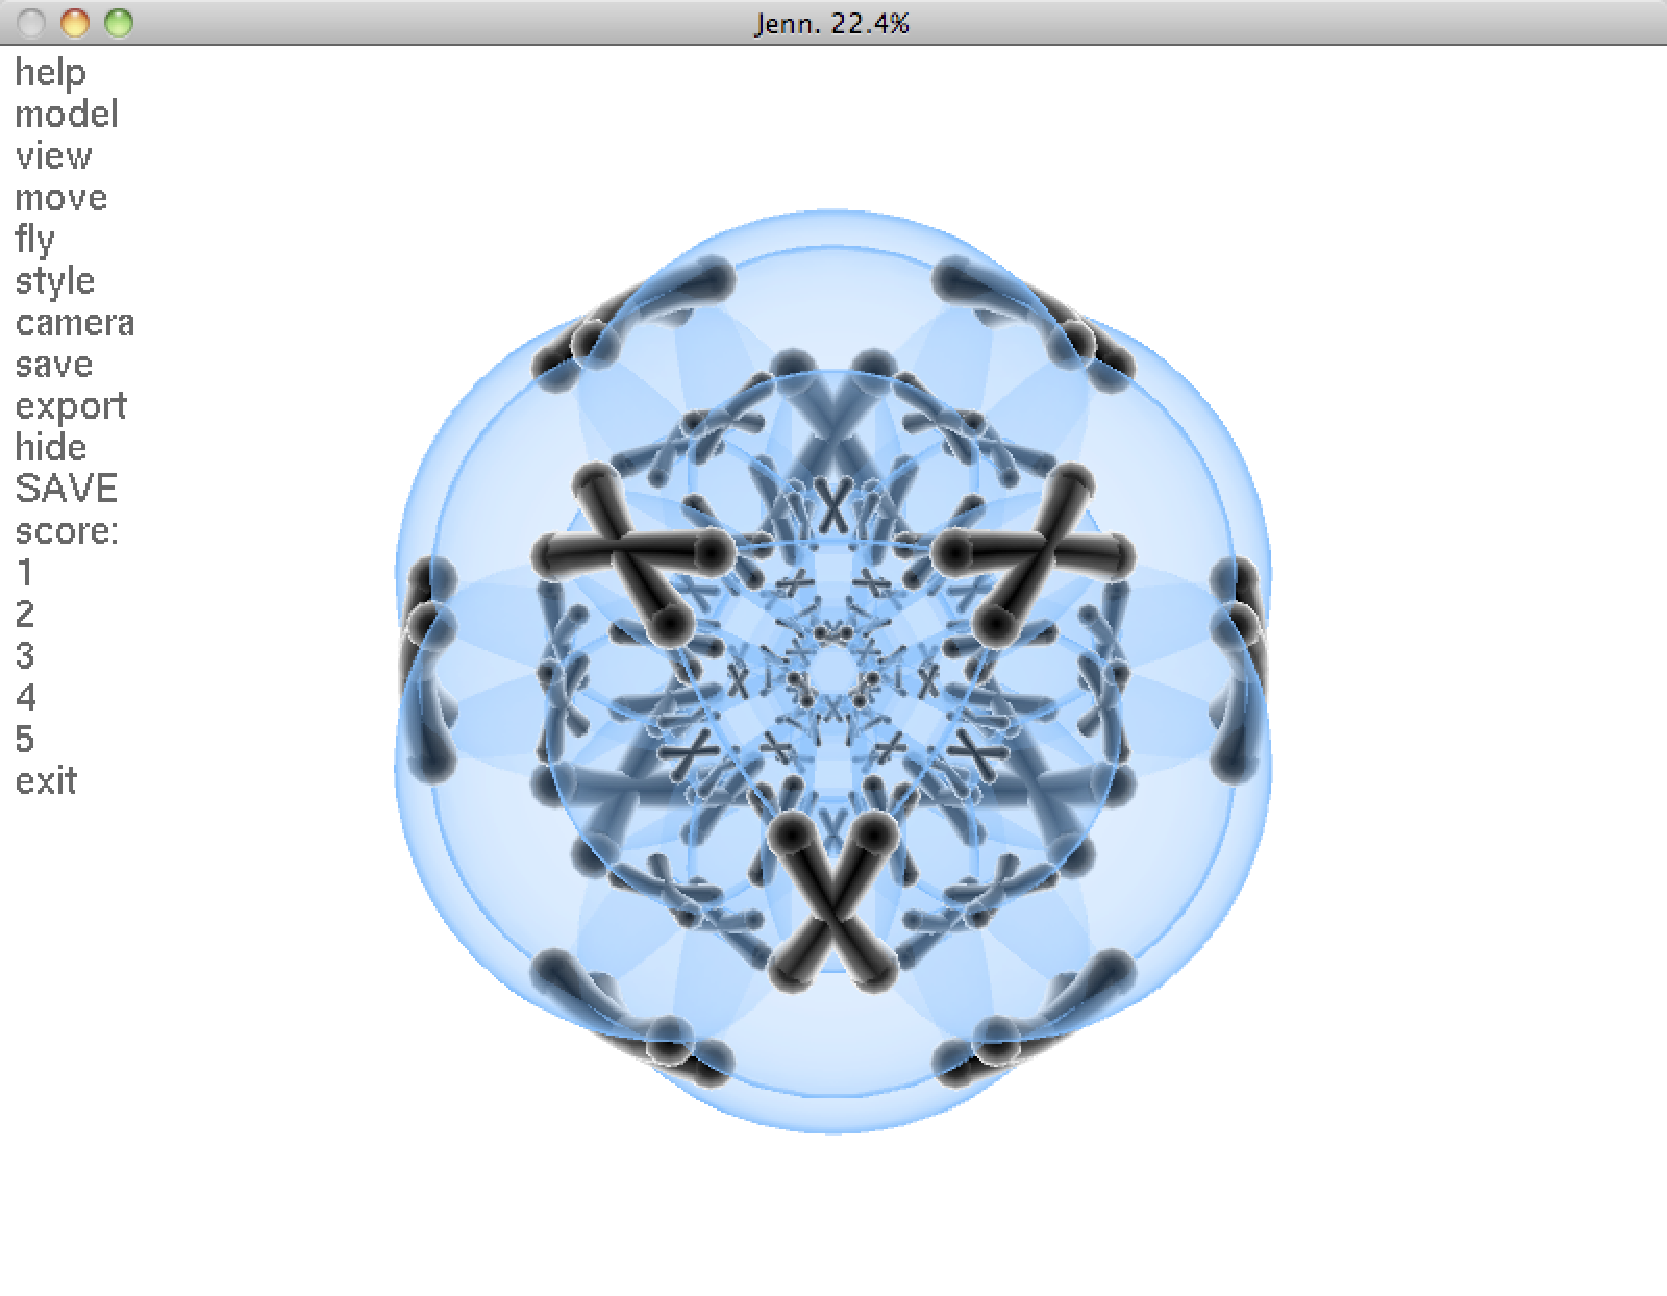
\includegraphics[width = .48\textwidth]{jennInterface1}
		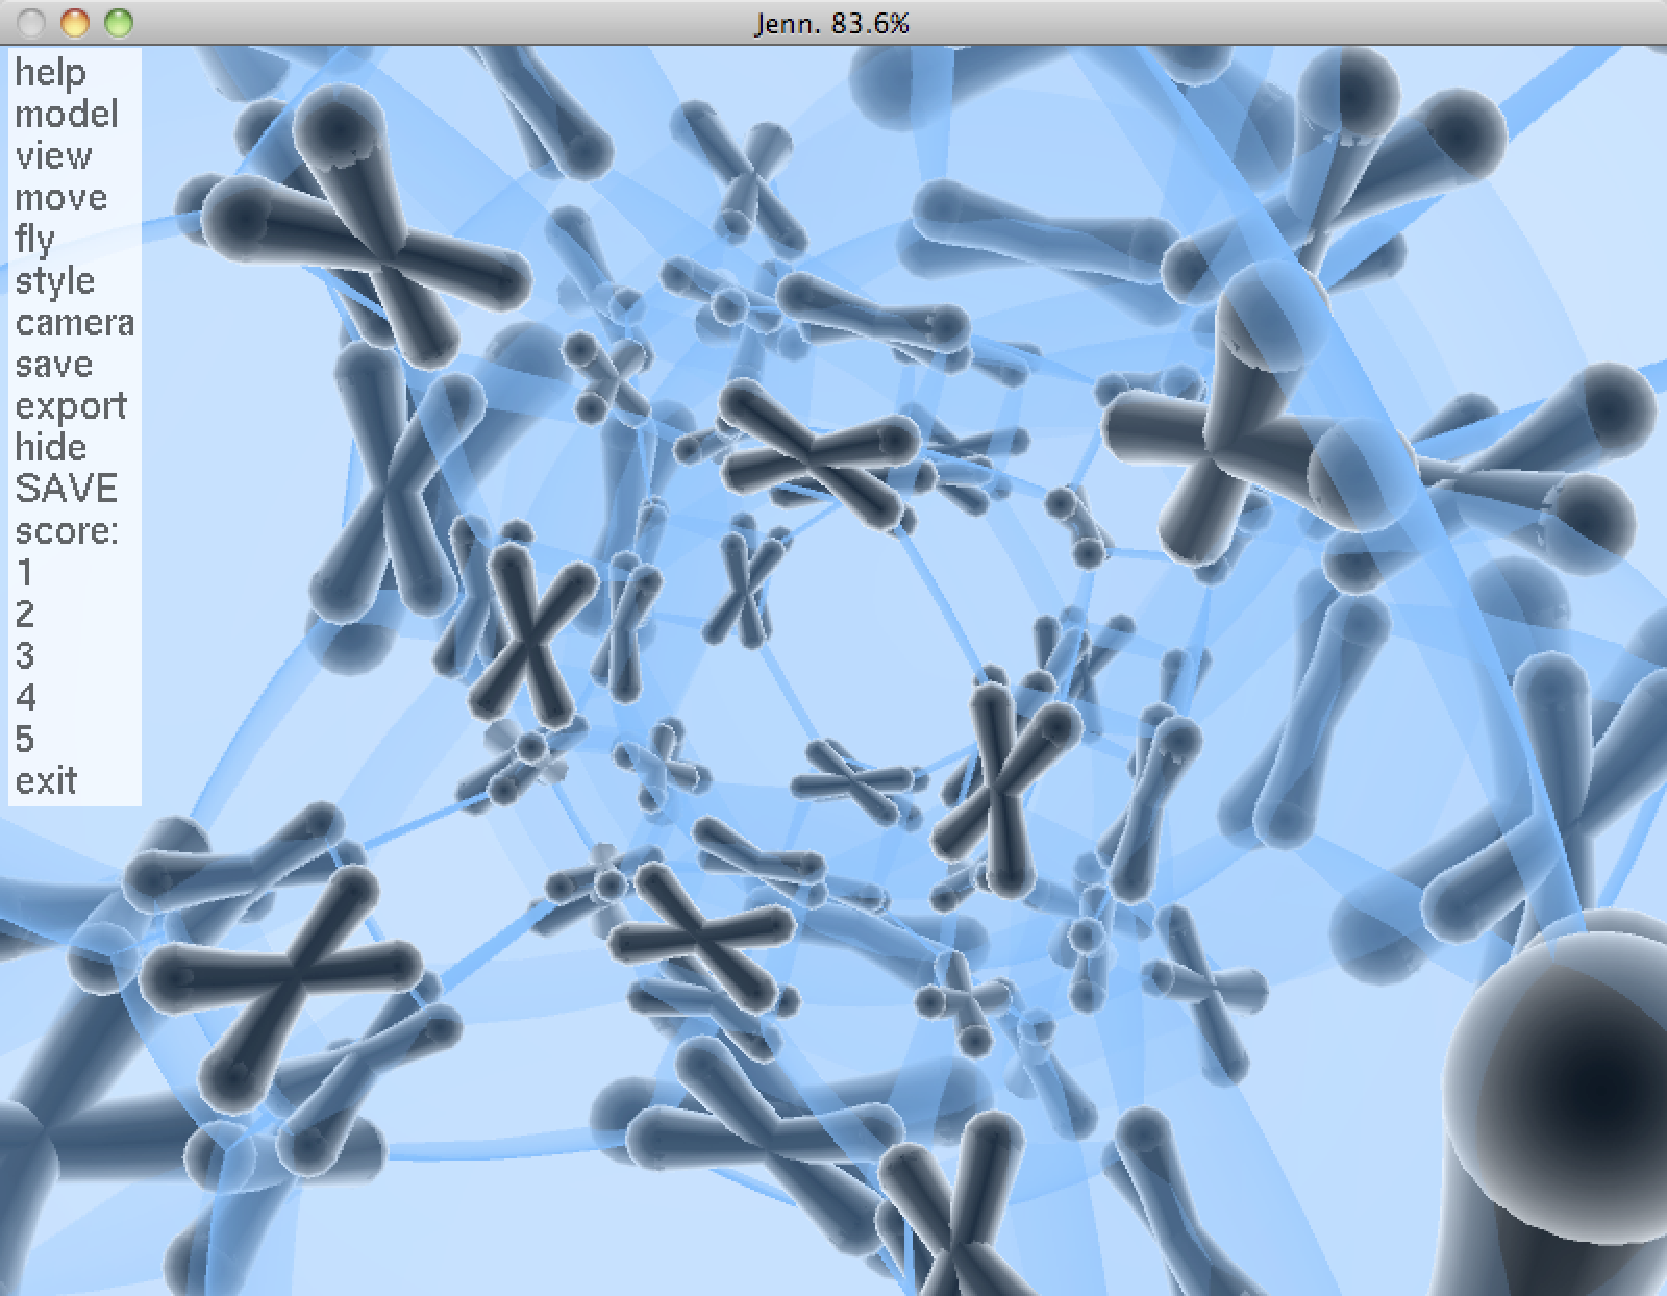
\includegraphics[width = .48\textwidth]{jennInterface2}
	\end{center}
	\caption{The Jenn3d interface, along with the extensions encoded. An
	example image is shown in the left; the same image, when zoomed in
	and rotated (right), can produce a dramatically different
	visualisation.}
	\label{interface}
\end{figure}

\subsubsection{Fitness and Typicality}

Table \ref{fittyp} shows the range of possible fitness and typicality scores.
Due to the complexity of the Todd-Coxeter algorithm, some visualisations are
impossible to generate, causing the Jenn3d software to crash\footnote{This can
be frustrating for the user; a quick way to deal with this problem (in a Mac
environment) is to leave the crash report window open, as new crash reports
will not be generated.}; as these might be close to correct (and potentially
attractive) visualisations, fitness and typicality scores of $0.5$ are
automatically attributed.

\begin{center}
	\begin{table}
	\caption{Fitness and Typicality scores, and events generating those
	scores; fitness values 1-5 are user supplied}
	\begin{tabular}{|l|c|c|}
		\hline
		Event & Fitness & Typicality\\
		\hline
		Unsuccessful GE mapping & 0.0 & 0\\
		\hline
		Non-convergence of Tedd-Coxeter algorithm & 0.5 & 0.5\\
		\hline
		Rejected visualisation & 1.0 & 1.0\\
		\hline
		Poor visualisation score & 2.0 & 1.0\\
		\hline
		Average visualisation score & 3.0 & 1.0\\
		\hline
		High visualisation score & 4.0 & 1.0\\
		\hline
		Visualisation remains in population unchanged & 5.0 & 1.0\\
		\hline
	\end{tabular}
	\label{fittyp}
	\end{table}
\end{center}

Ideally, the user has a large control of the evolutionary process, through the
fitness score. A fitness score of $1.0$, for example, guarantees that the
current visualisation is replaced by a random one in the next generation,
whereas a score of $5.0$ guarantees that the visualisation is passed unchanged
to the next generation, thus potentially being used as a seed for alternative,
similar visualisations (as per the scoring process proposed previously
\cite{nicolau2011a}).

The GA provided in the Java framework of the competition does not comply with
this scoring system, which limits to a small extent the user experience of the
system.

\section{Examples}
FIXME

FIXME: Mention that automatic export limits the user creativity, as a default
viewpoint is saved automatically to file. To really exploit the visual
complexity of the generated structures, user-selected viewpoints are much
nicer.

\bibliographystyle{plain}
\bibliography{jennWIAWReport}

\section*{Appendix A: Software details}

The Jenn3d software is written in C++, as is the GE mapping library used. In
order to integrate it in the Java framework provided for the competition, the
implementation of the \textit{Individual} (abstract) class in \texttt{Jenn.java} uses 
a system call to the C++ framework. This call is made in the \texttt{measureQuality()} 
method. The java code waits for an exit value from the system call and then reads 
from the file \texttt{fitness.txt} (created by the C++ code). The typicality value is then 
derived from the fitness value (as shown in Table \ref{fittyp}). Image generation is 
performed automatically by the C++ code when the user assigns a fitness score and the generated
file is stored in the \texttt{GEMapJenn} directory. This simplifies the operation of the
\texttt{export()} method in \texttt{Jenn.java} since all that is required is a file-copy
operation. Note that the PNG files from the \texttt{GEMapJenn} folder are not deleted so 
it may be necessary for the user to clean up these files to save on disk space.

It is important to note that in addition to the implementation of a new \texttt{domain} 
package, some minor changes to other code in the framework (to facilitate interactive evolution)
were also necessary. The superclass \texttt{Search.java} was modified to include a new field, 
\texttt{userQuit} and the main loops in subclasses \texttt{SearchGA.java} and \texttt{SearchMC.java} 
were modified to incorporate this value.

An ant buildfile has been supplied to aid with building and executing the code. To do this, call 
\texttt{ant run} from the JennWord directory. Note that before this can be executed, the 
C++ source code of the combined Jenn3d+GE mapper must be compiled first. To do
so, run \texttt{make} (\texttt{make -f makefile.mac} in a Mac environment) in
the \texttt{GEMapJenn} directory. In a Linux environment, installations of
the \texttt{libpng} and \texttt{freeglut3} libraries are required, whereas in a Mac 
a recent installation of XCode is required (the software has not been tested in a 
Windows environment).

\end{document}

